\section{Baggrund}
\begin{frame}{Robotteknologi indenfor kirurgi}{Udbredelse og fordele}
%\tableofcontents
\begin{minipage}[b]{0.55\linewidth}
\begin{block}{Incitament for projektet}
	\begin{itemize}
		\item Robotoperation
		\item Fordele for patient og kirurg
		\item Udbredelse i dag og i fremtiden
	\end{itemize}
\end{block}
\vspace{3mm}
\begin{block}{Semi-automatisering}
	\begin{itemize}
		\item Virtuelle fiksturer -- mindske risiko ved operation
		\item Garanti for patientsikkerhed
	\end{itemize}
\end{block}
\end{minipage}
	\hspace{0.1cm}
\begin{minipage}[b]{0.4\linewidth}
\begin{figure}[h]
\vspace{5mm}
\centering
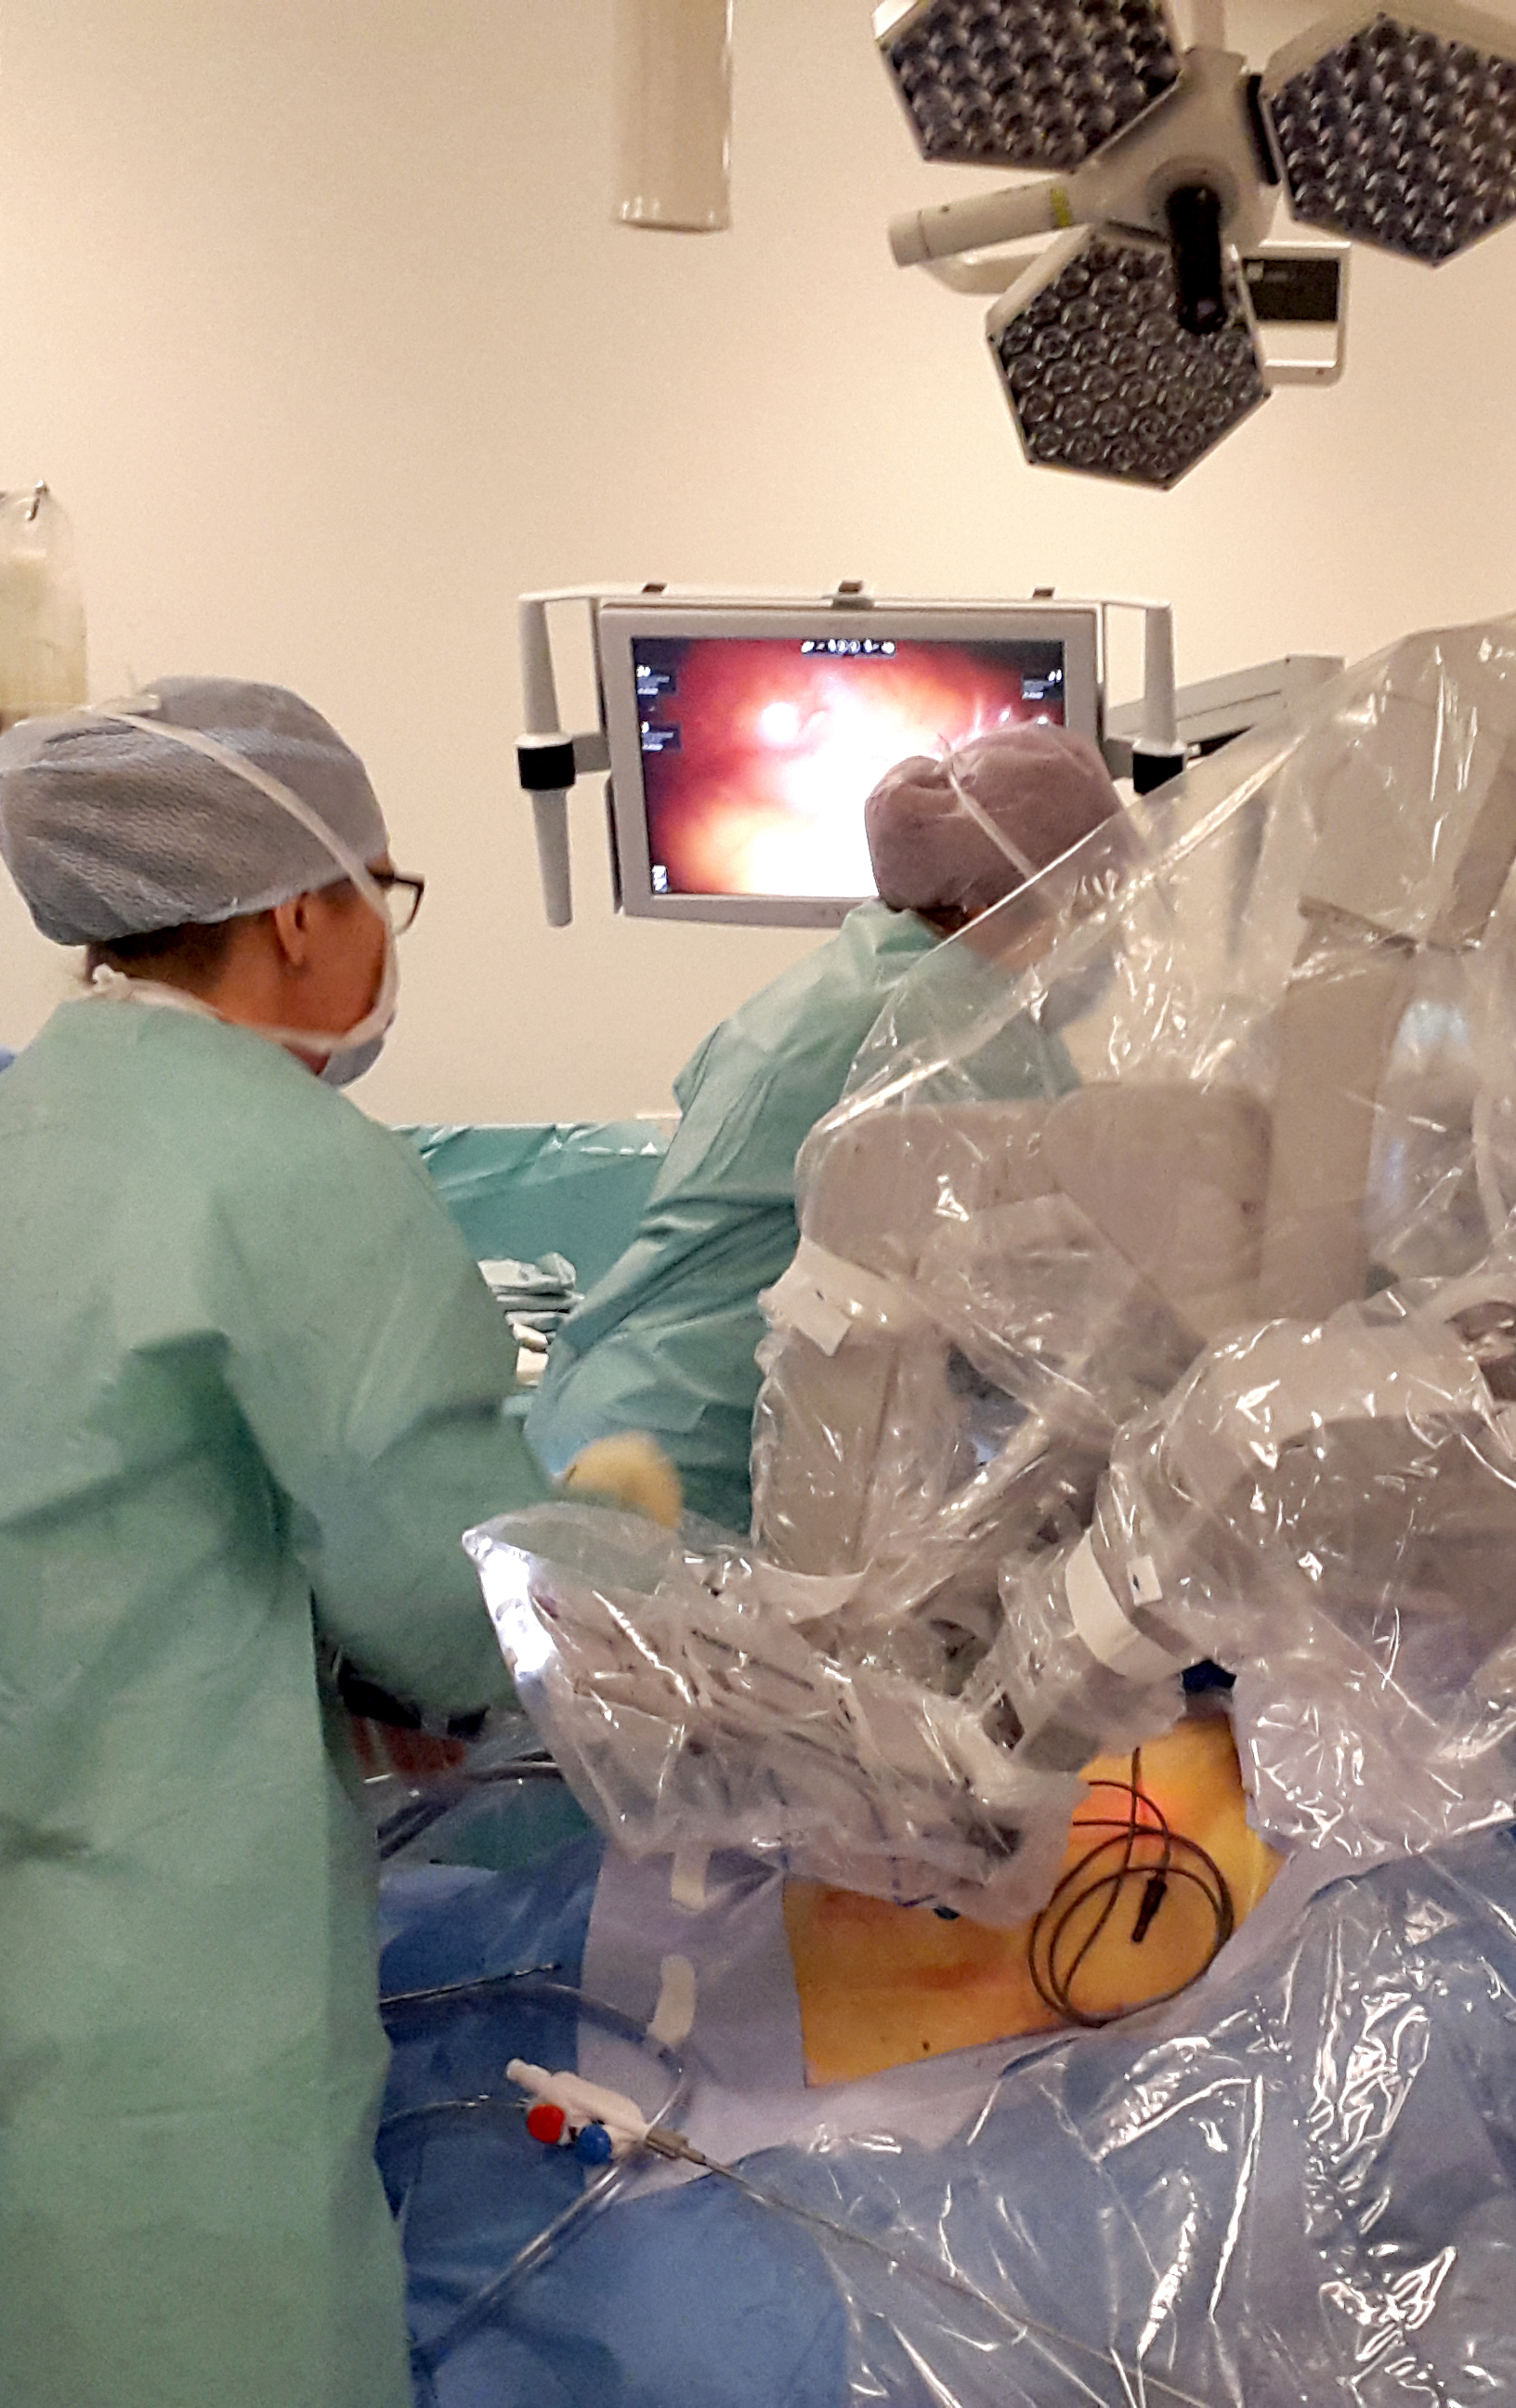
\includegraphics[width=1\textwidth]{20150526_102755.jpg}
\end{figure}
\end{minipage}
\vspace{1cm}
\end{frame}

\section{Kirurgirobot på AAU}
\begin{frame}{Kirurgirobotten på Aalborg Universitet}{Første-generations da Vinci-robot}
\begin{minipage}[b]{0.55\linewidth}
	\vspace{2mm}
\begin{block}{Modificeret da Vinci-robot}
	\begin{itemize}
		\item Patient-manipulator afkoblet fra master-konsol 
		\item \href{file:video/davinci_joints.mp4}{Videoklip af robotled}
		\item Implementation i ROS
	\end{itemize}
\end{block}
\vspace{-1mm}
\begin{block}{Fokus på sikkerhed}
	\begin{itemize}
		\item Barrierecertifikater til garanti af sikkerhed
		\item Design af sikkerhedsregulator vha. kontrolbarrierefunktioner
		\item Sikkerhedsanalyse for lukketsløjfesystemer
	\end{itemize}
\end{block}
\end{minipage}
\hspace{0.1cm}
%\vspace{-10mm}
\begin{minipage}[b]{0.4\linewidth}
	\begin{figure}[h]
%		\vspace*{-5mm}
		\centering
		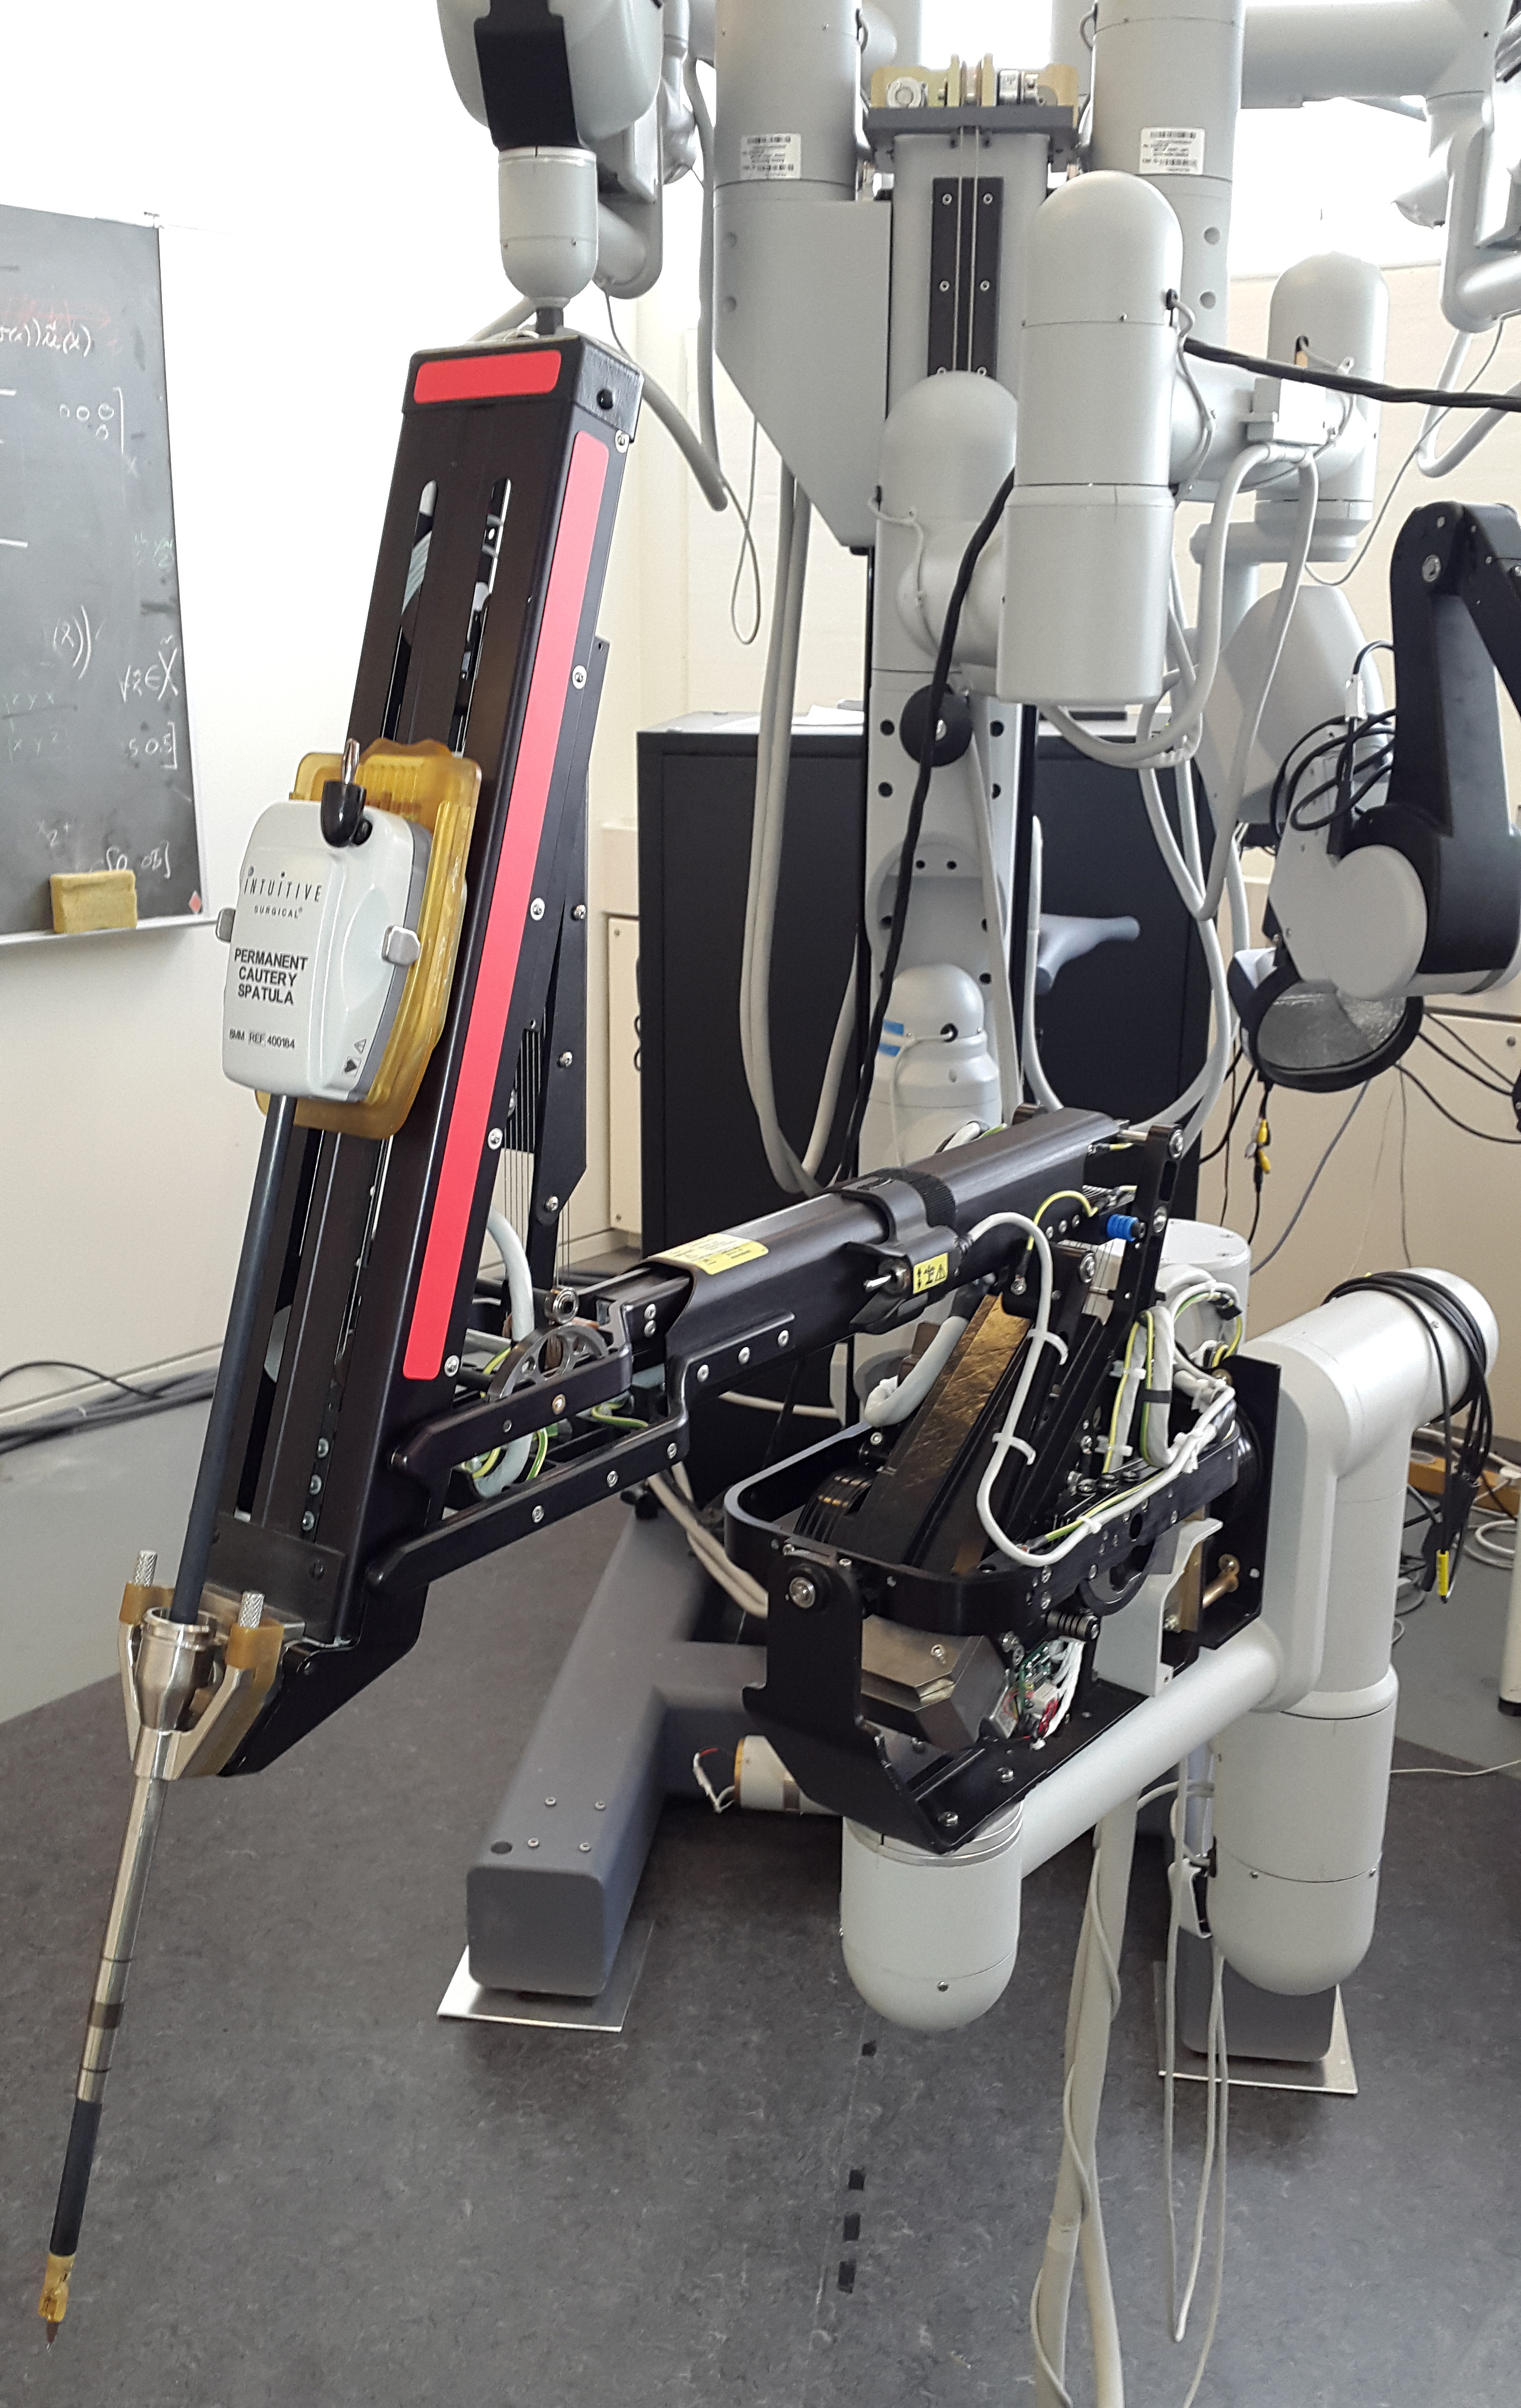
\includegraphics[width=1\textwidth]{20150517_120236.jpg}
	\end{figure}
\end{minipage}
\vspace{1cm}
\end{frame}

\section{Barrierecertifikater}
\begin{frame}{Barrierecertifikater}{Formelt bevis for garanteret sikkerhed}
\vspace{2mm}
\begin{block}{Definition af sikkerhed}
	\begin{itemize}
		\item Systemets tilstande er i $\mathcal{X}$
		\item Usikre tilstande er i $\mathcal{X}_u\subset\mathcal{X}$ og sikre tilstande i $\mathcal{X}_0\subseteq\mathcal{X}\setminus\mathcal{X}_u$
		\item Nulniveaukurven af $B(\textbf{x})$ danner  barriere mellem $\mathcal{X}_0$ og $\mathcal{X}_u$
	\end{itemize}
\end{block}
\begin{figure}[h]
	\centering
	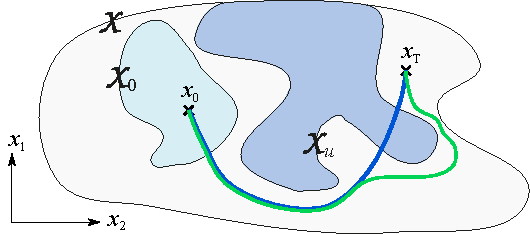
\includegraphics[width=0.8\textwidth]{safety.pdf}
\end{figure}
\vspace{1cm}
\end{frame}

\section{Kontroldesign}
\begin{frame}{Kontrolbarrierefunktioner (CBF)}{Konstruktion af CBF til design af sikkerhedsregulator}
	\vspace{2mm}
\begin{block}{To regulatorer}
	\begin{itemize}
		\item Lineær positionskontrol indenfor det sikre område $\mathcal{X}_0$
		\item Gradvis overgang til sikkerhedsregulator nær $\mathcal{X}_u$
		\item Designet vha. CLF så krav til sikkerhed bliver opfyldt
	\end{itemize}
\end{block}
\vspace{-2mm}
\begin{equation*}
u(\mathbf{x},\tilde{u})=\sigma(\mathbf{x})k_0(\mathbf{x})+(1-\sigma(\mathbf{x}))\tilde{u}(\mathbf{x})
\end{equation*}

\begin{figure}[h]
	\centering
	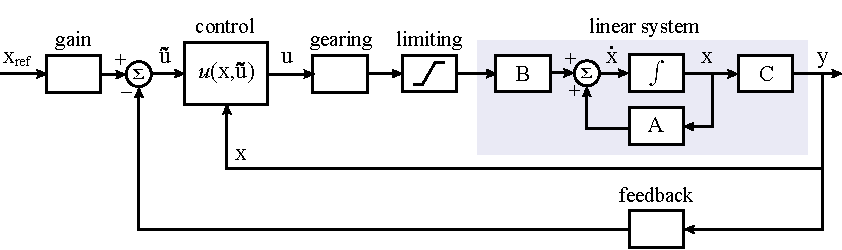
\includegraphics[width=0.9\textwidth]{control_system.pdf}
\end{figure}
	\vspace{5mm}
\end{frame}